\documentclass{article}
% We will use NIPS submission format
\usepackage{nips13submit_e,times}
% for hyperlinks
\usepackage{hyperref}
\usepackage{url}
% For figures
\usepackage{graphicx}
\usepackage{subfigure}
% math packages
\usepackage{amsmath}
\usepackage{amsfonts}
\usepackage{amsopn}
\usepackage{ifthen}
\usepackage{natbib}

\title{Machine Learning Project II by Group KATHMANDU}

\author{
  Jade Copet\\
  EPFL \\
  \texttt{jade.copet@epfl.com} \\
  \And
  Merlin Nimier David\\
  EPFL \\
  \texttt{merlin.nimier-david@epfl.com} \\
  \And
  Krishna Raj Sapkota\\
  EPFL \\
  \texttt{krishna.sapkota@epfl.com} \\
}

\nipsfinalcopy

\begin{document}
\maketitle



\begin{abstract}
\end{abstract}



\section{Song recommendation}

  \subsection{Dataset description}
  \textbf{Objective}: The song recommendation dataset represents the musical habits of users on a musical streaming service. We are given a large number of (user, artist, listening count) triplets, as well as a friendship graph encoding the connections between users. Our goal is to use this training data to perform:

  \begin{itemize}
    \item \textit{Weak} generalization: for existing users, predict the listening counts for unobserved (user, artist) pairs.
    \item \textit{Strong} generalization: for unknown users, predict the listening counts. We may use the friendship data.
  \end{itemize}

  \textbf{About the data}: The listening counts matrix $Y$ covers $1774$ users and $15085$ artists. It is very sparse, as we observe only $69617$ triplets (density of $0.2\%$). The friendship graph $G$ is given in the form of a symmetric $1774 \times 1774$ adjacency matrix, where $G_{i, j} = G_{j, i} = 1$ if users $i$ and $j$ are connected.\\

  Artists have listening counts ranging from $1$ to $2274039$, the most listened artist being Britney Spears (for some reason). Over all observations, before any outlier removal, the average count is 707 while the median count is 278.\\

  TODO: explain carefully how we handled unobserved data.

  \textbf{Error measure}: Both weak and strong prediction involve generating, for a given set of (user, artist) pairs, predicted listening counts. We use mean \textbf{RMSE} as our main error measure. Given a predicted triplets $\hat{Y}$, we compute the RMSE of the residuals on nonzero elements of the target sparse matrix $Y$.\\

  \subsection{Dataset analysis and preprocessing}
  Examining the dataset, we noticed that user $385$ had listened to artist $9162$ a whopping $352698$ times. Assuming an average song duration of $3$ minutes, user $385$ have supposedly spent the equivalent of two full years listening to \textit{Depeche Mode}. It was then necessary to remove such outliers before carrying out any learning.

  Several Machine Learning techniques rely on the assumption that data follows a Gaussian distribution. Applying a $\log$ transform to listening counts brought all counts back to a common scale.

  \begin{figure}[ht]
    \center
    \subfigure{
      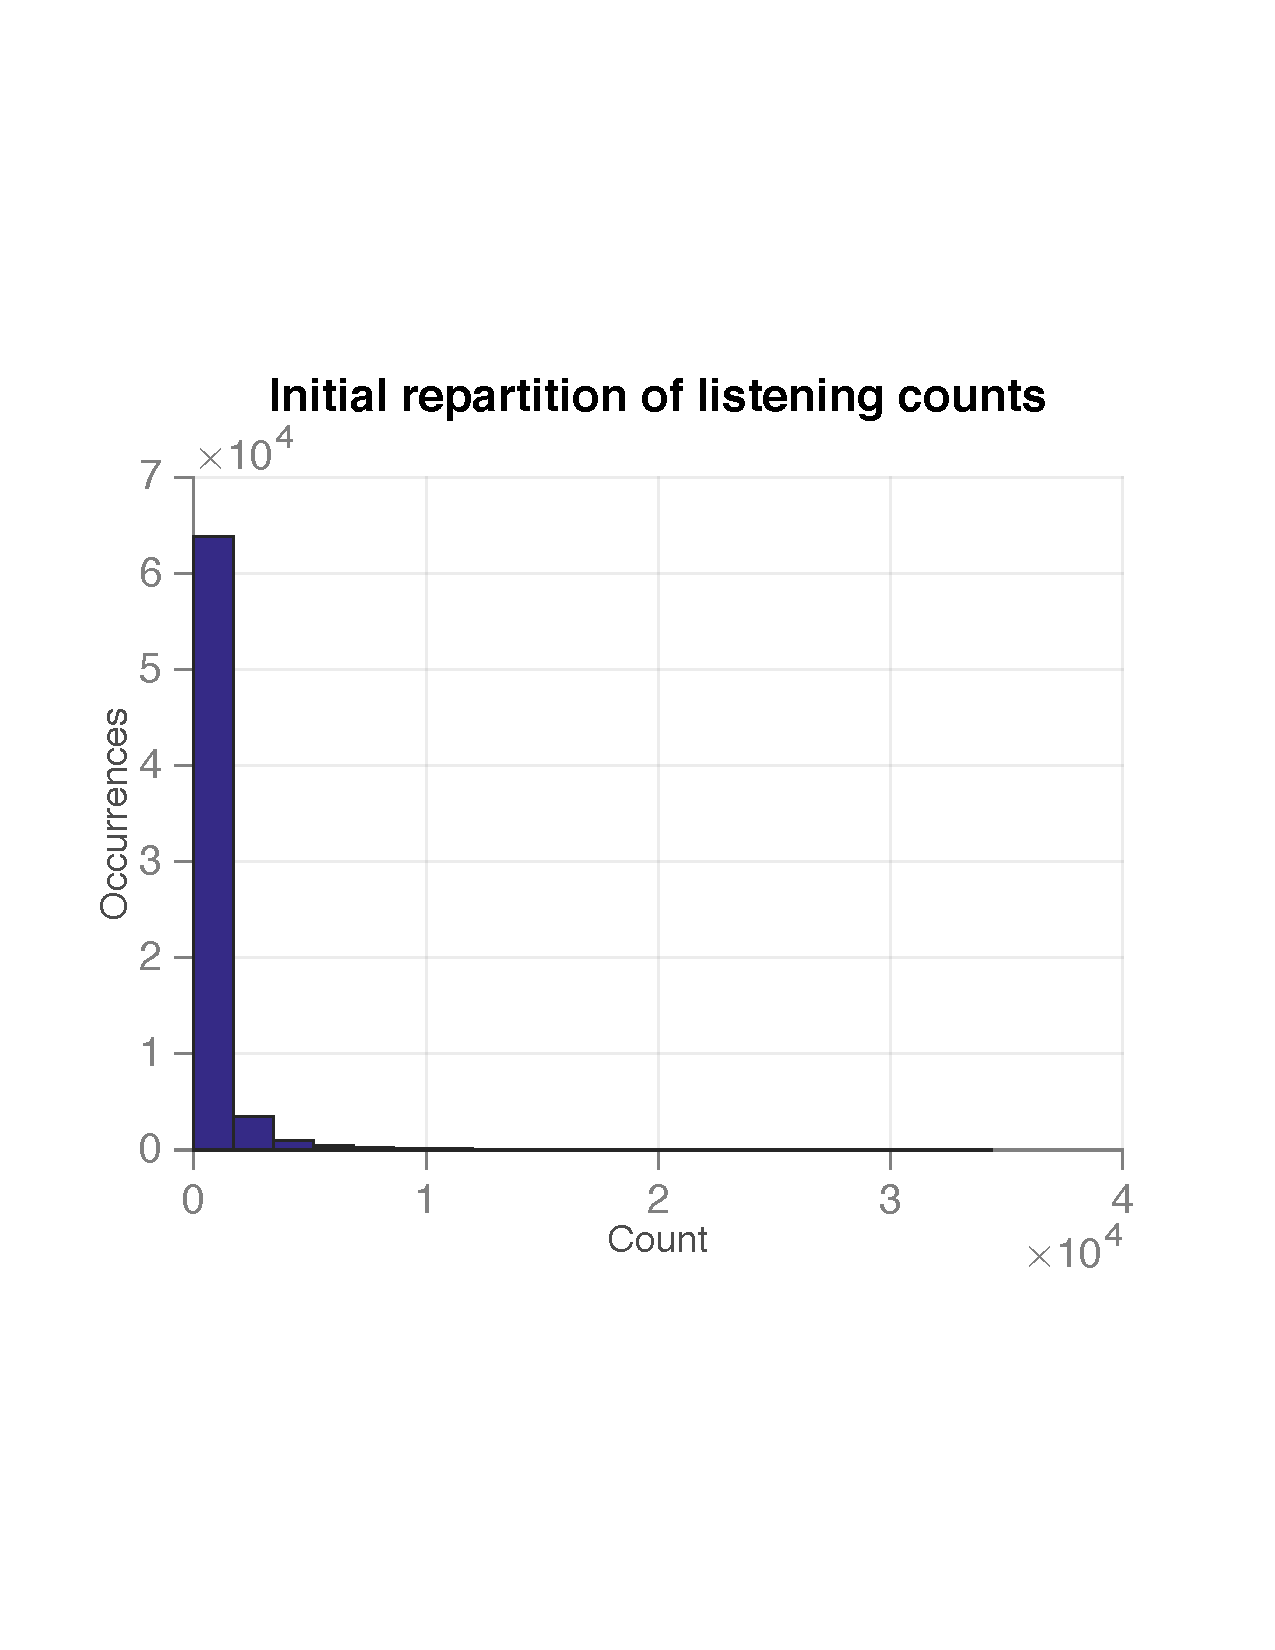
\includegraphics[width=2.5in]{figures/recommendation/unnormalized-counts.pdf}
    }
    \subfigure{
      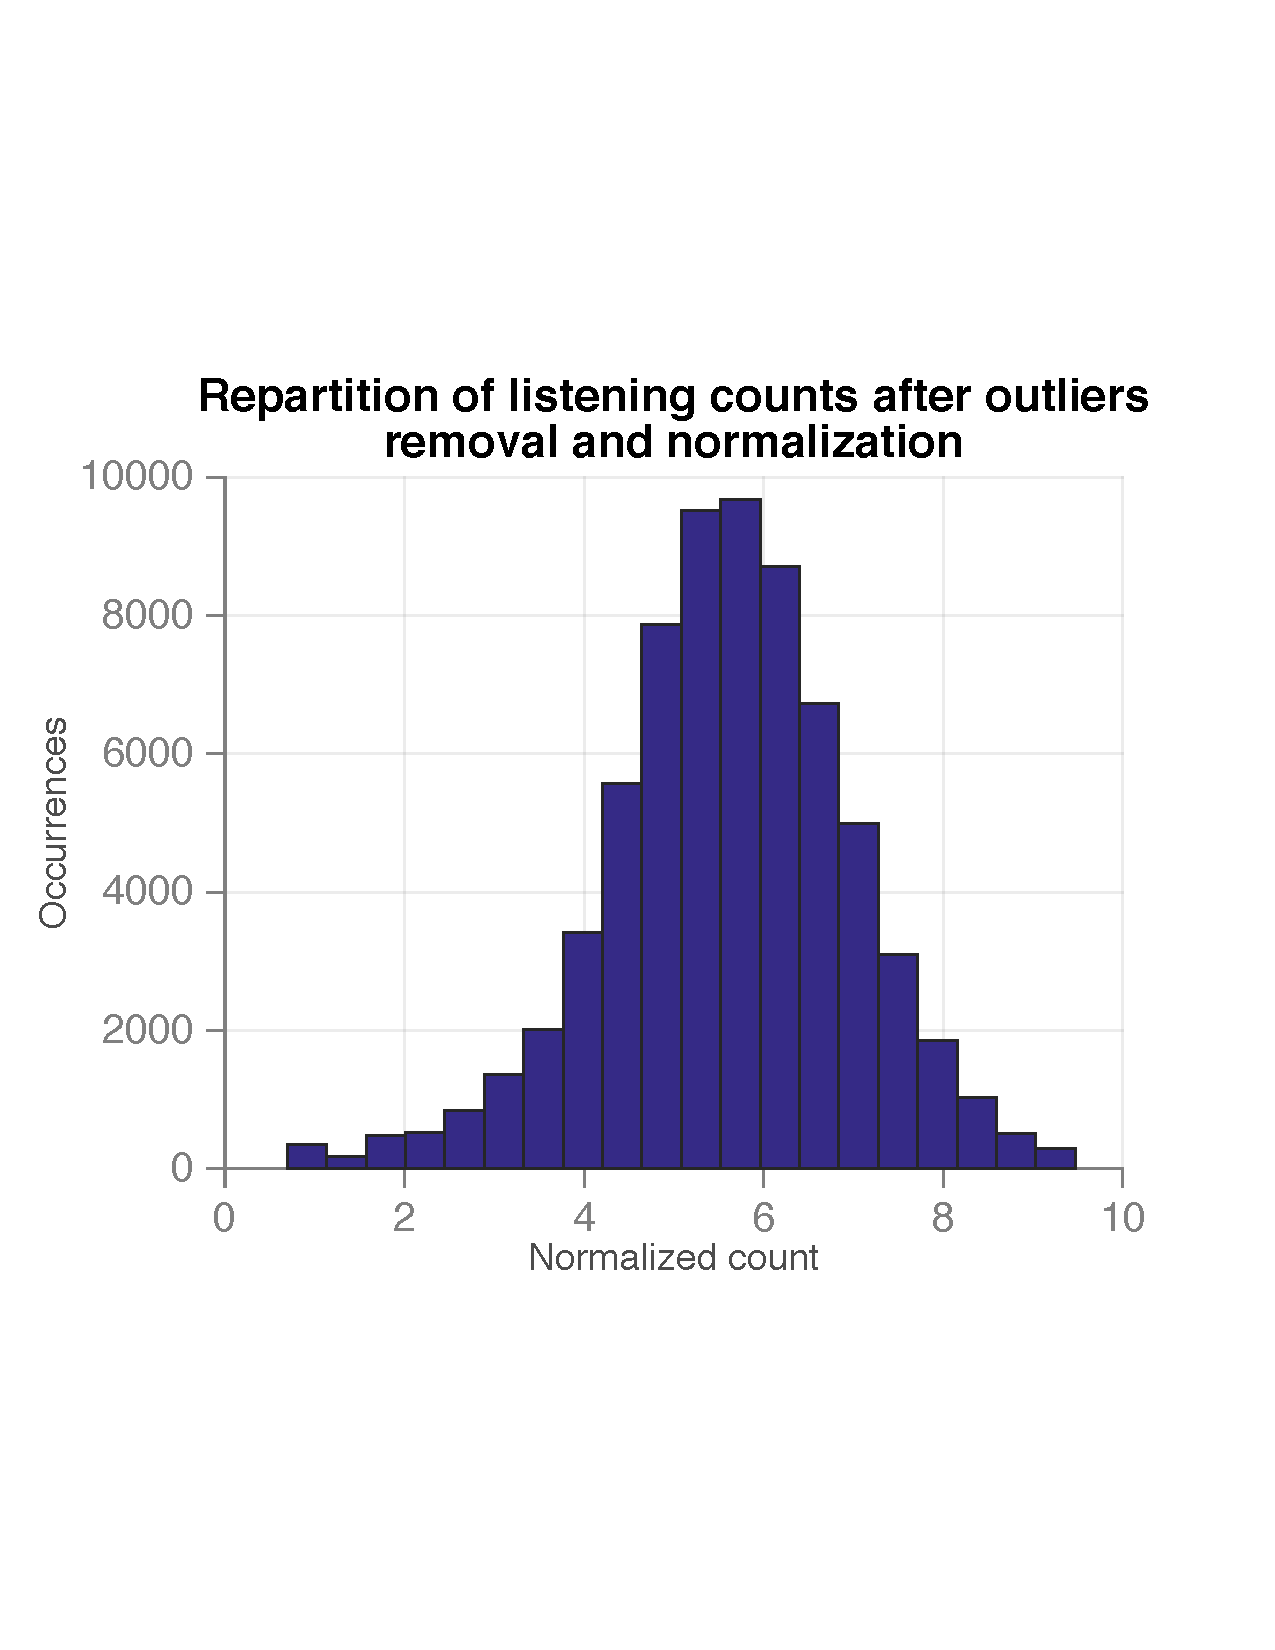
\includegraphics[width=2.5in]{figures/recommendation/normalized-counts.pdf}
    }
    \caption{Normalization makes listening counts distribution more Gaussian}
    \label{fig:recommendation-normalization}
  \end{figure}

  Finally, in order to test our models for both weak and strong predictions, we separated the training set in two ways:
  \begin{itemize}
    \item Entirely remove a proportion of users to use them as a strong prediction test set
    \item Withhold a proportion of the remaining (user, artist, listening count) triplets to use them as a weak prediction test set
  \end{itemize}

  \subsection{Feature transformations}

  \subsection{Final model and predictions}



\section{Image classification}

  \subsection{Dataset description}
  \textbf{Objective}: The people detection dataset consists of a set of images associated with a label that indicates whether there is a person or not in the image. Our goal is to predict whether people are present in unseen images.

  \textbf{Data characteristics}: The training set is composed of $8545$ examples. For each of these images, we are provided with the Histogram of Oriented Gradient (HOG) features generated with Piotr's toolbox. In order to work with the HOG features we convert them into a vector. Hence for each image we get a vector of dimensionality $9360$.

  The training dataset includes $1237$ positive examples (images with a person on it) encoded with the label $+1$ and $7308$ negative examples encoded with the label $-1$. The distribution is thus heavily skewed towards negative examples.

  \subsection{Performance Evaluation}
  As our dataset is imbalanced, we are relying on both True Positive (TP) and False Positive (FP) values as indicators of our performance. We are using the Receiver Operating Characteristics (ROC) measure and associated \textbf{ROC curves} to compare and evaluate our classifiers' performances. The ideal working point is the top-left corner of the ROC curve, where no misclassification is made.

  \subsection{Dataset pre-processing}
  From data exploratory analysis, we did not spot any obvious outlier. For all features, the examples of the training dataset lie between 2 and 3 standard deviations from the median.

  We tried several feature transformations: $\log$, $\exp$, $\sqrt{.}$ and $.^2$ of the input features but none of those seemed to enhance performance so we decided to keep working with the original features.\\
  TODO: check exp might be useful when using PCA (at least with 50 features)

  We normalized our features before using them for training.

  \subsection{Principal Component Analysis}
  Our features matrix is of dimensionality $9360$ for $8545$ examples which gives us a ``fat'' matrice. As several Machine Learning algorithms' time complexity grows fast with dimensionality, we applied a Principal Component Analysis (PCA) in order to work with lower dimensionality data. To do so, we used Piotr's \texttt{pca} implementation which proved to be faster than Matlab's default implementation. We decided to keep the $NTOREPLACE$ first principal components.\\
  TODO: Plot explained variance + find value by kCV ?.
  Using a reduced number of features also helps avoiding overfitting, as we are, to some extend, using only the signal (residing in the principal components).

  \subsection{Model selection}
  We learnt classifiers from several techniques and compared them to find the best performing model. We started with a simple Logistic Regression. Then, we applied Gaussian Processes classification using Rasmussen's GPML library, Support Vector Machines using LIBSVM toolbox, Neural Networks thanks to the Deep Learning toolbox, and finally Random Forests using Matlab's implementation.\\
  TODO: add \texttt{cite} references to all toolboxes.

  \textbf{General approach}:
   	\begin{itemize}
	   	\item Applying a default implementation of the model to normalized input data or reduced input data after applying PCA depending on computation complexity and performance of the algorithm.
    	\item Tuning model parameters: for parameters that seemed relevant, we chose a range of values to test on and find the best combination using to cross validation. As training the different models is rather slow, we used 3-fold cross validation. Other parameters were set manually. We plot learning curves and select parameters vlaues that maximize the average True Positive Rate (TPR) on the test set.
		  \item Validating the trained model using 3-fold cross-validation: we computed an average ROC curve over train and test data. We represent the curve with its 95\% confidence interval (see our \texttt{kCVfastROC} function).
  		\item Finally, we compare the candidate model with other classifiers plotting an ROC Curve for each of them.
	\end{itemize}

  \textbf{Logistic Regression}: Since it can be seen as a single-layer Neural Network, we used the Deep Learning toolbox. We added a regularization term (see below for details).

  \textbf{Gaussian Processes}: Having a large number of data examples in our training set, we used ``large scale'' GP classification from Rasmussen's GPML library. It relies on low-rank and diagonal approximation to the exact covariance using induction points. Solving a classification problem, we opted for a logistic function as a likelihood function. We did not have specific intuition about the prior distribution so we used a constant 0-mean prior. We selected a squared exponential covariance with isometric distance measure \texttt{covSEiso} rather than the squared exponential. While yielding comparable performance, the former uses only two hyper-parameters, in contrast with the latter which needs $D+1$ hyper parameters and thus might be prone to overfitting. Finally we chose Laplace approximation to infer on our data because of its reasonable computation time (as opposed to Expectation-Propagation).\\
  TODO: May need to explain how each hyperparam works... [WHY ALL PARAMETERS?]

  \textbf{Support Vectors Machines}: We experimented with different kernels: linear, polynomial and Radial Basis Function (RBF). As the polynomial and RBF kernels are more complex models their computational complexity is much higher than the linear one. Hence we applied SVM with those kernels on our low-rank approximation data. We retained the RBF kernel because it was giving the best performance results and then we select the best smoothness parameter $\gamma$ over a range of possible values through cross validation.\\
  TODO: figures (comparing the kernels, learning curves for the selected kernel).

  \textbf{Random Forests}: TODO
  \begin{itemize}
    \item number of trees
    \item fraction of variables in random bagging
    \item minLeaf
    \item Learning parameters with kCV
  \end{itemize}

  \textbf{Neural Networks}: We applied a 2-layered Neural Network on our full-dimension data. We were able to tune the number of activation functions on each layer as well as its type. A sigmoid activation function gives better results than the $\tanh$ function.\\
  TODO: why?\\
  To avoid overfitting, we leveraged two regularization methods:
  \begin{itemize}
   	\item Applying weight decay on the second layer (corresponding to Tikhonov regularization)
	  \item Defining a ``dropout fraction'', which removes randomly some activation functions during the training\\
    TODO: reference the paper + check formulation of what it does
  \end{itemize}
	The best combination of weight decay and dropout fraction parameters were selected from ranges of parameters using cross-validation as described in the general approach section.\\
  TODO: ref, give the ranges, learning curves

  \textbf{Models comparison}: TODO\\
  \begin{itemize}
    \item Plot ROC Curves with the different models, compare, check variance (Random guessing as a base model for comparison)\\
    \item Discuss which was difficult or not
  \end{itemize}

  \subsection{Final model and predictions}
  TODO


\section{Summary}
  Sparse matrix representation made manipulation less straightforward and required us to learn a few new techniques.

  \subsubsection*{Acknowledgments}

  \subsubsection*{References}



\end{document}
